\documentclass[10pt,journal,compsoc]{IEEEtran}
\usepackage{graphicx, soul} 
\usepackage{soul} % soul pachage must be removed when the paper is ready
\usepackage{colortbl} % Biblioteca para el color
\usepackage{color} % Biblioteca para el color
\usepackage{xcolor} % Biblioteca para el color

\usepackage{listings}
\usepackage{hyperref}

%% A number of IDs used in authentication protocols
\newcommand{\lnk}{;}
\newcommand{\QR}{Qr}

%% Operators
\newcommand{\keysFor}{\textsf{keysFor}\;}
\newcommand{\invKey}{\textsf{invKey}\;}

%% Message items

\newcommand{\Agent}{\textsf{Agent}\;}
\newcommand{\Number}{\textsf{Number}\;}
\newcommand{\Key}{\textsf{Key}\;}
\newcommand{\Nonce}{\textsf{Nonce}\;}
\newcommand{\Hash}{\textsf{Hash}\;}
\newcommand{\Crypt}{\textsf{Crypt}\;}
\newcommand{\Xor}{\textsf{Xor}}

%% Rôles

\newcommand{\initiator}{\textrm{initiator}} 
\newcommand{\responder}{\textrm{responder}}

%% Events and messages

\newcommand{\msg}{\mathsf{msg}}

%% Agents, server, etc.
\newcommand{\Friend}{\textsf{Friend}\;}
\newcommand{\Spy}{\textsf{Spy}}
\newcommand{\Server}{\textsf{M}}
\newcommand{\ServerW}{\textsf{M}_{W}}
\newcommand{\Servera}{\textsf{S}_{CA}}
\newcommand{\Client}{\textsf{C}}
\newcommand{\server}{\textsf{Server}\;}

%% Event operators

\newcommand{\knows}{\textsf{knows}\;}
\newcommand{\knowsSpy}{\textsf{knows}\,_{\textsf{\tiny Spy}}\:}
\newcommand{\knowsF}{\textsf{knows}\,_{\textsf{\tiny Friend}}\:}
\newcommand{\initState}{\textsf{initState}\;}
\newcommand{\bad}{\textsf{bad}\;}

%% def operator
\newcommand{\Def}{\stackrel{\rm def}{=}}

%% BAN constructors


%% Needham constructors
\newcommand{\nsPub}{\textsf{ns\_public}\;} 
\newcommand{\evsone}{\textsf{evs1}}
\newcommand{\evstwo}{\textsf{evs2}}
\newcommand{\evsthree}{\textsf{evs3}}


\newcommand{\fat}[1]{\left\{\hspace*{-0.03in}\left|{#1}\right|\hspace*{-0.03in}\right\}}

\newcommand{\lfat}[1]{\left\{\!\arrowvert{#1}\right.}
\newcommand{\rfat}[1]{\left.{#1}\arrowvert\!\right\}}

%\newcommand{\fat}[1]{\lbrace\!|{#1}|\;\,\,\!\!\!\!\rbrace}
\newcommand{\cons}{\,\#\,}

%Stega constructors
\newcommand{\As}{\textsf{AE}\;}

%% equal2Eyes operator
\newcommand{\eqToEyes}{\stackrel{\odot}{\approx}}

\ifCLASSOPTIONcompsoc
 \usepackage[nocompress]{cite}
\else
  \usepackage{cite}
\fi

\ifCLASSINFOpdf
\else
\fi
\hyphenation{Blockchain and smart contracts}

\begin{document}
        \newcommand{\blockchaincarnetwork}{\textit{vehicle blockchain network~}}
        \newcommand{\duda}[1]{\textcolor{red}{\textit{#1}}}

        %
% paper title
% Titles are generally capitalized except for words such as a, an, and, as,
% at, but, by, for, in, nor, of, on, or, the, to and up, which are usually
% not capitalized unless they are the first or last word of the title.
% Linebreaks \\ can be used within to get better formatting as desired.
% Do not put math or special symbols in the title.

%\title{A Framework of Protocols to solve Car Purchase Fraud Through Blockchain Platform}
%\title{A Model to solve Vehicle Purchase Fraud Through Blockchain Platform}
\title{A Distributed Model to Store Vehicle Transaction Records Through Blockchain Platform}
%
%
% author names and IEEE memberships
% note positions of commas and nonbreaking spaces ( ~ ) LaTeX will not break
% a structure at a ~ so this keeps an author's name from being broken across
% two lines.
% use \thanks{} to gain access to the first footnote area
% a separate \thanks must be used for each paragraph as LaTeX2e's \thanks
% was not built to handle multiple paragraphs
%
%
%\IEEEcompsocitemizethanks is a special \thanks that produces the bulleted
% lists the Computer Society journals use for "first footnote" author
% affiliations. Use \IEEEcompsocthanksitem which works much like \item
% for each affiliation group. When not in compsoc mode,
% \IEEEcompsocitemizethanks becomes like \thanks and
% \IEEEcompsocthanksitem becomes a line break with idention. This
% facilitates dual compilation, although admittedly the differences in the
% desired content of \author between the different types of papers makes a
% one-size-fits-all approach a daunting prospect. For instance, compsoc 
% journal papers have the author affiliations above the "Manuscript
% received ..."  text while in non-compsoc journals this is reversed. Sigh.

\author{XXXXX,~\IEEEmembership{Member,~IEEE,}
        XXXXX,~\IEEEmembership{Fellow,~OSA,}
        and~XXXX~XXXX,~\IEEEmembership{Life~Fellow,~IEEE}% <-this % stops a space
\IEEEcompsocitemizethanks{\IEEEcompsocthanksitem M. Shell was with the Department
of Electrical and Computer Engineering, Georgia Institute of Technology, Atlanta,
GA, 30332.\protect\\
% note need leading \protect in front of \\ to get a newline within \thanks as
% \\ is fragile and will error, could use \hfil\break instead.
E-mail: see http://www.michaelshell.org/contact.html
\IEEEcompsocthanksitem J. Doe and J. Doe are with Anonymous University.}% <-this % stops an unwanted space
\thanks{Manuscript received April 19, 2005; revised August 26, 2015.}}

% note the % following the last \IEEEmembership and also \thanks - 
% these prevent an unwanted space from occurring between the last author name
% and the end of the author line. i.e., if you had this:
% 
% \author{....lastname \thanks{...} \thanks{...} }
%                     ^------------^------------^----Do not want these spaces!
%
% a space would be appended to the last name and could cause every name on that
% line to be shifted left slightly. This is one of those "LaTeX things". For
% instance, "\textbf{A} \textbf{B}" will typeset as "A B" not "AB". To get
% "AB" then you have to do: "\textbf{A}\textbf{B}"
% \thanks is no different in this regard, so shield the last } of each \thanks
% that ends a line with a % and do not let a space in before the next \thanks.
% Spaces after \IEEEmembership other than the last one are OK (and needed) as
% you are supposed to have spaces between the names. For what it is worth,
% this is a minor point as most people would not even notice if the said evil
% space somehow managed to creep in.



% The paper headers
\markboth{Journal of \LaTeX\ Class Files,~Vol.~XX, No.~X, August~2018}%
{Shell \MakeLowercase{\textit{et al.}}: Bare Demo of IEEEtran.cls for Computer Society Journals}
% The only time the second header will appear is for the odd numbered pages
% after the title page when using the twoside option.
% 
% *** Note that you probably will NOT want to include the author's ***
% *** name in the headers of peer review papers.                   ***
% You can use \ifCLASSOPTIONpeerreview for conditional compilation here if
% you desire.



% The publisher's ID mark at the bottom of the page is less important with
% Computer Society journal papers as those publications place the marks
% outside of the main text columns and, therefore, unlike regular IEEE
% journals, the available text space is not reduced by their presence.
% If you want to put a publisher's ID mark on the page you can do it like
% this:
%\IEEEpubid{0000--0000/00\$00.00~\copyright~2015 IEEE}
% or like this to get the Computer Society new two part style.
%\IEEEpubid{\makebox[\columnwidth]{\hfill 0000--0000/00/\$00.00~\copyright~2015 IEEE}%
%\hspace{\columnsep}\makebox[\columnwidth]{Published by the IEEE Computer Society\hfill}}
% Remember, if you use this you must call \IEEEpubidadjcol in the second
% column for its text to clear the IEEEpubid mark (Computer Society jorunal
% papers don't need this extra clearance.)



% use for special paper notices
%\IEEEspecialpapernotice{(Invited Paper)}



% for Computer Society papers, we must declare the abstract and index terms
% PRIOR to the title within the \IEEEtitleabstractindextext IEEEtran
% command as these need to go into the title area created by \maketitle.
% As a general rule, do not put math, special symbols or citations
% in the abstract or keywords.
\IEEEtitleabstractindextext{%
\begin{abstract}

    %Blockchain technology, from its emergence until now, has been applied to several projects and 
%not just for cryptocurrencies. 
%Although this technology has been used for several challenges, to our knowledge, there are no 
%records of having applied it to smart properties in vehicles.
%In this work, we present a transaction based solution to handle motorized vehicles ownership 
%and provenance. 
%The solution is based on a distributed model using smart properties and blockchain technologies,  
%which offers a secure and useful system where transactions can be requested to handle, 
%validate and update the vehicle information. 
%The model includes the specification of various client-server security protocols.  
%The client can have different roles accordingly to the relationship it has with the 
%physical property and it can get services and request transactions;
%meanwhile the \blockchaincarnetwork  acts as the server entity. 
%%Some transaction examples are shown. 
%We believe that our proposal can contribute to reduce frauds and increase the trend of 
%paperless culture that is strongly being promoted in recent years.

We present a transaction based solution to handle motorized vehicles ownership 
and provenance over a distributed model using smart contracts,  
including the specification of client-server security protocols,
roles, services, transactions and the \blockchaincarnetwork acting as server.
Our proposal will reduce frauds and increase the trend of paperless culture.
\end{abstract}

% Note that keywords are not normally used for peerreview papers.
\begin{IEEEkeywords}
Smart contract, Smart property, Blockchain, Cloud Computing, Security Protocols.
\end{IEEEkeywords}}


% make the title area
\maketitle


% To allow for easy dual compilation without having to reenter the
% abstract/keywords data, the \IEEEtitleabstractindextext text will
% not be used in maketitle, but will appear (i.e., to be "transported")
% here as \IEEEdisplaynontitleabstractindextext when the compsoc 
% or transmag modes are not selected <OR> if conference mode is selected 
% - because all conference papers position the abstract like regular
% papers do.
\IEEEdisplaynontitleabstractindextext
% \IEEEdisplaynontitleabstractindextext has no effect when using
% compsoc or transmag under a non-conference mode.



% For peer review papers, you can put extra information on the cover
% page as needed:
% \ifCLASSOPTIONpeerreview
% \begin{center} \bfseries EDICS Category: 3-BBND \end{center}
% \fi
%
% For peerreview papers, this IEEEtran command inserts a page break and
% creates the second title. It will be ignored for other modes.
\IEEEpeerreviewmaketitle




        
        %\tableofcontents    % this line must be removed
        
       % \section{Introduction}
The paperless culture extends throughout the world. 
From the birth of the scanner to the invention of cloud computing, 
technology has been making its way into business processes 
with the aim of facilitating operations and reducing the use of paper, 
for both economic and environmental reasons. 

To do that, 
companies who seek to become paperless, can automate their processes with a 
minimum use of paper and contributing to a higher automation.
This is not a complete process and in some cases is not even encouraged.
Even today, 
in some communities where an electronic bill is required when selling goods, 
it has to be printed afterwards and then officially signed, 
via holograms or stamps, 
for it to become a legal proof. 
The combination of electronic and physical documents introduces some application problems, 
like a lack of clarity in the process of passing ownership.
Specially troublesome is the case when the goods are expensive, like automobiles.
Sometimes, a car is the most valuable possession a person has, 
making the selling process a subject of constant scrutiny 
because if a fraud is committed in the exchange, 
the affected can lose a big part of its patrimony.

The paperless culture extends throughout the world. From the birth of the scanner to the invention 
of cloud computing, technology has been making its way into business processes with the aim of
facilitating operations and reducing the use of paper, for both economic and environmental reasons. 
To do that, companies seek to become paperless that can automate their processes with the 
minimum use of paper and with the highest automation.

In response to this, around the world there is an initiative for electronic invoice instead of the physical paper. 
Our interest is related to some problems that this initiative has caused in the 
purchase process of vehicles in Mexico. This is described as follows:

From 2011, paper bills stopped being legal proof of ownership for cars. An electronic bill had to be generated by a seller in order to legally report a car selling took place.
The process of the selling is described bellow:
\begin{enumerate}
    \item The buyer checks that no legal problems are involved with the vehicle. An online check can be done with the plates numbers. 
    \item The buyer makes the car payment
    \item The seller generates an electronic bill for the value of the car and acknowledges payment from the buyer.
    \item The seller gives possession of the car to the buyer.
    \item The change of ownership is notified to the city government. 
    \item The old plates are discarded and a new set of plates is given the new owner.
\end{enumerate}

This work flow has a vulnerability between steps $2$ and $3$. The electronic bill generated in step $2$ can be generated even without the existence of a physical car. A malicious seller could generate multiple bills and give them to multiple people before they realize the car doesn't exist physically. A certain level of \textit{trust} must exist between buyer and seller for the exchange to happen. And this \textit{trust} can be maligned. 

This fraud is specially common on car sales between private owners for a couple reasons. The first one is the high value of this commodity, which makes it a low risks - high stakes trade-off for fraudsters. The other one comes with the definition of car: A portable, efficient, and maneuverable transportation vehicle that can be easily removed from the transaction scene and hidden afterwards.

Due to the lack of immediate retaliation available to the criminal, he has a time frame where the fraud could be repeated multiple times, even if finally, the car exchange takes place with an Innocent buyer afterwards.

To solve our challenge, smart properties  is a recent technology that can be used to this. Smart property is those whose ownership is controlled via block chain technology using smart contracts~\cite{Tapscott2016}. Examples could include physical property such as vehicles, phones or houses. A smart contract is a computer protocol intended to digitally facilitate, verify, or enforce the negotiation or performance of a contract, using transactions. These transactions are trackable and irreversible. 

So, we propose a model to solve vehicle purchase fraud through blockchain network platform. In this paper we present our model consisting in including a QR code in vehicles by Dealerships and it can be read by users who can use it to do transactions through \blockchaincarnetwork. 
We have used Alice and Bob notation to explain our general model. We think that our proposal can be applied to other countries around the world who are looking for having a digital ecosystem and better
control over the transaction history that a vehicle can have throughout its life.

The rest of the paper is organized as follows: 
Section~\ref{sec:TheoreticalFramework} describes the notation used 
throughout the document and expounds the blockchain and smart contracts, 
which constitutes a fundamental part of our work; 
Section~\ref{sec:outline} presents the framework we are proposing. 
%the invoice supply-chain provenance. 
Section~\ref{sec:Services} explains step by step the proposal.
Finally, our conclusions are given.
        %\subsection{Fraud Description}
From 2011, paper bills stopped being legal proof of ownership for cars. An electronic bill had to be generated by a seller in order to legally report a car selling took place.
The process of the selling is described bellow:
\begin{itemize}
    \item The buyer checks that no legal problems are involved with the vehicle. An online check can be done with the plates numbers. 
    \item The buyer makes the car payment
    \item The seller generates an electronic bill for the value of the car and acknowledges payment from the buyer.
    \item The seller gives possession of the car to the buyer.
    \item The change of ownership is notified to the city government. 
    \item The old plates are discarded and a new set of plates is given the new owner.
\end{itemize}

This work flow has a vulnerability between steps $2$ and $3$. The electronic bill generated in step $2$ can be generated even without the existence of a physical car. A malicious seller could generate multiple bills and give them to multiple people before they realize the car doesn't exist physically. A certain level of \textit{trust} must exist between buyer and seller for the exchange to happen. And this \textit{trust} can be maligned. 

This fraud is specially common on car sales between private owners for a couple reasons. The first one is the high value of this commodity, which makes it a low risks - high stakes trade-off for fraudsters. The other one comes with the definition of car: A portable, efficient, and maneuverable transportation vehicle that can be easily removed from the transaction scene and hidden afterwards.

Due to the lack of immediate retaliation available to the criminal, he has a time frame where the fraud could be repeated multiple times, even if finally, the car exchange takes place with an Innocent buyer afterwards.
        %\section{Client roles}

According to the permissions the clients should have, there will be three defined roles for them:

\begin{enumerate}
    \item Querier
    \item Owner
    \item Helper
    \item Law enforcer
\end{enumerate}

The querier will have permissions sufficient to interact with the system in order to query and obtain information on the vehicle. This permissions will be granted to the querier once the client is able to establish a secure channel.

Every car will have one and only one owner at a given time. The owner will be the only client that has permission to trade ownership. 


The helper role is a client who receives a temporal permission from the owner to set one transaction on the block-chain. The time frame for the temporal permission will be allotted by the owner of the car. The car owner will set a special transaction to give the helper the permission. 
The helper role will be used for transactions that change the value of the property. This will include official services, mechanical adjustments, big aesthetic modifications and insurance payments.

The law enforce roles will have the ability to change the value of the car when the vehicle is involved in legal situations. It won’t need the permission of the owner to modify the status.
        \section{Introduction}
The paperless culture extends throughout the world. 
From the birth of the scanner to the invention of cloud computing, 
technology has been making its way into business processes 
with the aim of facilitating operations and reducing the use of paper, 
for both economic and environmental reasons. 

To do that, 
companies who seek to become paperless, can automate their processes with a 
minimum use of paper and contributing to a higher automation.
This is not a complete process and in some cases is not even encouraged.
Even today, 
in some communities where an electronic bill is required when selling goods, 
it has to be printed afterwards and then officially signed, 
via holograms or stamps, 
for it to become a legal proof. 
The combination of electronic and physical documents introduces some application problems, 
like a lack of clarity in the process of passing ownership.
Specially troublesome is the case when the goods are expensive, like automobiles.
Sometimes, a car is the most valuable possession a person has, 
making the selling process a subject of constant scrutiny 
because if a fraud is committed in the exchange, 
the affected can lose a big part of its patrimony.

The paperless culture extends throughout the world. From the birth of the scanner to the invention 
of cloud computing, technology has been making its way into business processes with the aim of
facilitating operations and reducing the use of paper, for both economic and environmental reasons. 
To do that, companies seek to become paperless that can automate their processes with the 
minimum use of paper and with the highest automation.

In response to this, around the world there is an initiative for electronic invoice instead of the physical paper. 
Our interest is related to some problems that this initiative has caused in the 
purchase process of vehicles in Mexico. This is described as follows:

From 2011, paper bills stopped being legal proof of ownership for cars. An electronic bill had to be generated by a seller in order to legally report a car selling took place.
The process of the selling is described bellow:
\begin{enumerate}
    \item The buyer checks that no legal problems are involved with the vehicle. An online check can be done with the plates numbers. 
    \item The buyer makes the car payment
    \item The seller generates an electronic bill for the value of the car and acknowledges payment from the buyer.
    \item The seller gives possession of the car to the buyer.
    \item The change of ownership is notified to the city government. 
    \item The old plates are discarded and a new set of plates is given the new owner.
\end{enumerate}

This work flow has a vulnerability between steps $2$ and $3$. The electronic bill generated in step $2$ can be generated even without the existence of a physical car. A malicious seller could generate multiple bills and give them to multiple people before they realize the car doesn't exist physically. A certain level of \textit{trust} must exist between buyer and seller for the exchange to happen. And this \textit{trust} can be maligned. 

This fraud is specially common on car sales between private owners for a couple reasons. The first one is the high value of this commodity, which makes it a low risks - high stakes trade-off for fraudsters. The other one comes with the definition of car: A portable, efficient, and maneuverable transportation vehicle that can be easily removed from the transaction scene and hidden afterwards.

Due to the lack of immediate retaliation available to the criminal, he has a time frame where the fraud could be repeated multiple times, even if finally, the car exchange takes place with an Innocent buyer afterwards.

To solve our challenge, smart properties  is a recent technology that can be used to this. Smart property is those whose ownership is controlled via block chain technology using smart contracts~\cite{Tapscott2016}. Examples could include physical property such as vehicles, phones or houses. A smart contract is a computer protocol intended to digitally facilitate, verify, or enforce the negotiation or performance of a contract, using transactions. These transactions are trackable and irreversible. 

So, we propose a model to solve vehicle purchase fraud through blockchain network platform. In this paper we present our model consisting in including a QR code in vehicles by Dealerships and it can be read by users who can use it to do transactions through \blockchaincarnetwork. 
We have used Alice and Bob notation to explain our general model. We think that our proposal can be applied to other countries around the world who are looking for having a digital ecosystem and better
control over the transaction history that a vehicle can have throughout its life.

The rest of the paper is organized as follows: 
Section~\ref{sec:TheoreticalFramework} describes the notation used 
throughout the document and expounds the blockchain and smart contracts, 
which constitutes a fundamental part of our work; 
Section~\ref{sec:outline} presents the framework we are proposing. 
%the invoice supply-chain provenance. 
Section~\ref{sec:Services} explains step by step the proposal.
Finally, our conclusions are given.
        \section{Background}
\label{sec:background}

\subsection{Blockchain}

Blockchain technology can be abstracted to recall a series of blocks chained in series. In this abstraction, each block of the blockchain represents an object that records a transaction and the chaining is obtained by referencing the previously last block. Blockchain is a transaction record keeping platform that tries to attack a series of problems contained in other similar purpose platforms. It achieves its purposes by having the following features \cite{block}:

\begin{itemize}
\item Immutable: It is not possible a given block.
\item Distributed system: Multiple copies of the blockchain exist among its members.
\item No centralized server: Blockchain does not depend on a central authority that dominates the system.            
\end{itemize}
Even though all these features are desired, when blockchain is mentioned as a solution is because of decentralization. Thus, giving control of the system to networks where the main beneficiaries are the users without necessarily having a government figure interested in controlling those exchanges, or where the users prefer to not involve third parties, due to the costs involved or the cumbersomeness of the extra steps required. 

The distribution and immutability of the chain also removes the trust component of a transaction \cite{iot}, i.e. making it a secure way to exchange titles of property between strangers.

\subsection{Data provenance}
Cloud computing allows the existence of digital representations of phyisical world objects in a permanent way, independent of a single copy existing on a specific location. This digital representation can contain information of the whole life cycle of the object, its accountability and historical changes. Specifically among cloud technologies, blockchain allows for the continuous existence of the digital representations introducing security aspects like traceability and resistance to unwanted modifications. Implementations have been made to preserve digital representations \cite{provchain}. Kim and Laskowski\cite{ontology} show an approach using Ethereum technology to propose ontologies that can represent knowledge provenance. The blockchain approach is having a great momentum in the data provenance medium for it theoretical strengths in security and data protection. Neisse et al. \cite{europe} give this a push by proposing enforcement of smart contracts to fulfill legal obligations of personal data over data controllers and processsors in Europe using blockchain. Blockchain provenance is not limited to storage information. Smart contracts inside the transactions allow for programmable interactive environments \cite{ramachandran} where the blockchain will be enriched with valid data and binding transactions every time something interesting happens to the physical part of the object.
\subsection{Smart Contracts}

A smart contract are a series of self-executing computer code that is fired when a transaction is trying to complete. These lines of code are part of the blockchain and allows for a series of conditions between the sender and receiver of the transaction to be completed before it succeeds. The whole process is completely automated without external help, requiring only the participation of the interested parties and the blockchain network.

The transaction itself can be a representation of a legal enforcement, and when used this way, should offer tamper-proofing to remove the possibility of bad use by either part. \cite{templates}

The existence of smart contracts over a blockchain expand the use cases of this revolutionary technology above its original use as a currency system \cite{nakamoto} \cite{uses}. Among multiple platforms that allow smart contract interactions \cite{sense}\cite{lazy}, Ethereum \cite{ethereum }as a platform also provides a full system where users can run custom-scripted code inside their transactions, embracing the idea of smart contracts over a decentralized medium. \cite{hawk}




\subsection{Fraud Description}
From 2011, paper bills stopped being legal proof of ownership for cars. An electronic bill had to be generated by a seller in order to legally report a car selling took place.
The process of the selling is described bellow:
\begin{itemize}
    \item The buyer checks that no legal problems are involved with the vehicle. An online check can be done with the plates numbers. 
    \item The buyer makes the car payment
    \item The seller generates an electronic bill for the value of the car and acknowledges payment from the buyer.
    \item The seller gives possession of the car to the buyer.
    \item The change of ownership is notified to the city government. 
    \item The old plates are discarded and a new set of plates is given the new owner.
\end{itemize}

This work flow has a vulnerability between steps $2$ and $3$. The electronic bill generated in step $2$ can be generated even without the existence of a physical car. A malicious seller could generate multiple bills and give them to multiple people before they realize the car doesn't exist physically. A certain level of \textit{trust} must exist between buyer and seller for the exchange to happen. And this \textit{trust} can be maligned. 

This fraud is specially common on car sales between private owners for a couple reasons. The first one is the high value of this commodity, which makes it a low risks - high stakes trade-off for fraudsters. The other one comes with the definition of car: A portable, efficient, and maneuverable transportation vehicle that can be easily removed from the transaction scene and hidden afterwards.

Due to the lack of immediate retaliation available to the criminal, he has a time frame where the fraud could be repeated multiple times, even if finally, the car exchange takes place with an Innocent buyer afterwards.

\subsection{Notation}
%As you can see, our stages imply the use of cryptography,  and security protocol techniques. 
% The following two sub-sections describe the notation used in the rest of
% the document. 

% \subsubsection{Host level notation}
% \label{sec:hostLevel}
Cryptography has two main mechanisms:
\begin{itemize}
  \item Symmetric cryptography, the same key is used to encode and
    decode a message; by convention, symbol $\fat{m}_{K_{AB}}$ will be
    used to denote that a message $m$ has been cyphered under the key
    $K_{AB}$, which agents $A$ and $B$ know. \footnote{An agent is a 
        computer process that uses the client-server technology to 
        establish a network communication. Sometimes we will use the 
        terms agent or client indistinctly.} 
  \item Asymmetric cryptography, two keys are used to encode and
    decode messages; an agent (e.g. $A$) has a key pair
    (public $K_{pub(A)}$ and private $K_{priv(A)}$). One key used to
    encode and the other one to decode (reciprocally); usually, key
    $K_{priv(A)}$ is kept in secret. 
\end{itemize}
Table~\ref{table:conventions} summarizes previous notations:
\begin{table}[htb]
\footnotesize
\begin{center}
\caption{Conventions in types of messages and agents}
\label{table:conventions}
\begin{tabular}{|l|l|}
\hline
{\bf Abbreviation}& {\bf Description}                                   \\\hline\hline
$C$                 &  Agent, Client or Smartphone application able to \\
                    &  establish communication with other agent.         \\ 
$\Server$           &  A trusted agent, best known as trusted Miner-Server      \\
$K$                 &  Symmetric key                                      \\
$K_{AB}$            &  Symmetric key shared with agents $A$ and $B$       \\
$K_{pub(A)}$        &  Public key of Agent $A$                            \\
$K_{priv(A)}$       &  Private key of Agent $A$                           \\
$\fat{m}_{K}$       &  Message $m$ cyphered under key $K$                 \\
$m1\lnk m2$         &  $m1$ and $m2$ are concatenated using symbol $\lnk$ \\
$[m_1:: m_2]$       &  A list o messages, $m_1$ representing the first element\\
$N_a$, $N_b$, $N_c$ &  Nonces, which are random unguessable numbers      \\
                    &  never been used before.                           \\ \hline \hline
\end{tabular}
\end{center}
\end{table}
\normalsize

% \subsubsection{Notation at network level}
% \label{sec:networkLevel}
For easy representation issues we will use Alice and Bob notation to 
describe Client-Server communication, see table~\ref{table:NetConventions}.
%three views (see ): i) initial knowledge;
%ii) message sending and message reception; and iii) the local process
%representation.
\begin{table}[htb]
\footnotesize
\begin{center}
\caption{Conventions in network level}
\label{table:NetConventions}
\begin{tabular}{|l|l|}
\hline
{\bf Abbreviation}                      & {\bf Description}                    \\\hline\hline
\textbf{Initial knowledge:}             &                                      \\
$A : ik$                                &  Initially agent $A$ knows $ik$.    \\ \hline 
\textbf{Message Sending and Receiving:} &  At step $n$ agent $A$ sends         \\ 
$n. A \rightarrow B: m$                 &  message $m$ to agent $B$,\\
                                        &  which $B$ receives.      \\ \hline 
$n. A\rightarrow B: m$                  &  message $m2$ was generated \\ 
\hspace{5mm}\textbf{Local process:}     &  Between steps $n$ and $n2$,    \\ 
\hspace{5mm}$m2 = f(m)$                 &  by $B$ as a local process \\ 
$n2. B\rightarrow A: m2$                &  generated from $f(m)$.     \\ \hline 
\textbf{Broadcast:}                     &  $A$ broadcasts message to agents\\ 
$A \rightarrow [B, C, D]: m$            &  $B$, $C$ and $D$.\\ \hline \hline 
\end{tabular}
\end{center}
\end{table}
\normalsize


$$$$

 %added by JC
        \section{Outline and Notation}
\label{sec:outline}

%This section describes in words our general framework and describes
%the general notation used to explain the formalism.

In general there exists some characteristics we are looking for vehicles:
a) Provenance,
b) Transparency with respects to purchase sale,
c) Traceability with history transactions, owners and legal situations.

To achieve that, we propose a model illustrated in Figure~\ref{fig:flowChartFramework}.


\subsection{Outline for the Framework}
\label{subsec:proposal}
Figure~\ref{fig:flowChartFramework} illustrates a context diagram denoting
the general stages a client must follow to get or set information about a car. 
\begin{figure}[bt]
 %\begin{center}
  \centering
    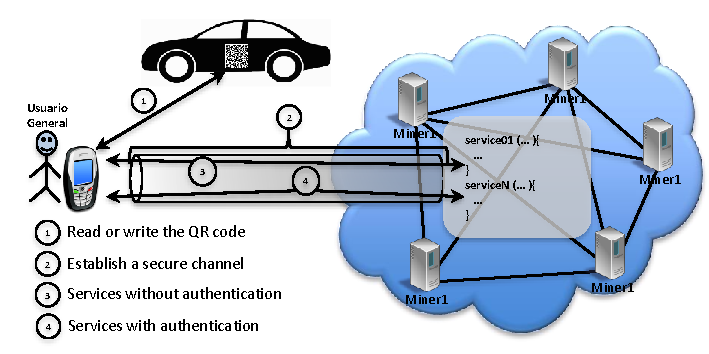
\includegraphics[scale=0.7]{images/gralScheme.pdf}
        \caption{Diagram about the use of the framework from the client view}
    \label{fig:flowChartFramework}
 % \end{center}
\end{figure}

\begin{itemize}
  \item \textbf{Stage I} consists in getting information of a car through reading
    a QR code or setting the QR code (this is the case when a company manufactures a car 
    and generates the genesis block.
  \item \textbf{Stage II} consists in establishing a secure channel. We
    have used the TLS protocol because it is the standard in the
    e-commerce and it has been subject to a lot of verification proofs.  
  \item \textbf{Stage III} consists in to obtain services, authentication
    is not required.   
  \item \textbf{Stage IV:} consists in to obtain services or set transactions, 
    authentication is required.  
\end{itemize}

\subsection{Notation}
%As you can see, our stages imply the use of cryptography,  and security protocol techniques. 
% The following two sub-sections describe the notation used in the rest of
% the document. 

% \subsubsection{Host level notation}
% \label{sec:hostLevel}
Cryptography has two main mechanisms:
\begin{itemize}
  \item Symmetric cryptography, the same key is used to encode and
    decode a message; by convention, symbol $\fat{m}_{K_{AB}}$ will be
    used to denote that a message $m$ has been cyphered under the key
    $K_{AB}$, which agents $A$ and $B$ know. \footnote{An agent is a 
        computer process that uses the client-server technology to 
        establish a network communication. Sometimes we will use the 
        terms agent or client indistinctly.} 
  \item Asymmetric cryptography, two keys are used to encode and
    decode messages; an agent (e.g. $A$) has a key pair
    (public $K_{pub(A)}$ and private $K_{priv(A)}$). One key used to
    encode and the other one to decode (reciprocally); usually, key
    $K_{priv(A)}$ is kept in secret. 
\end{itemize}
Table~\ref{table:conventions} summarizes previous notations:
\begin{table}[htb]
\footnotesize
\begin{center}
\caption{Conventions in types of messages and agents}
\label{table:conventions}
\begin{tabular}{|l|l|}
\hline
{\bf Abbreviation}& {\bf Description}                                   \\\hline\hline
$A$, $B$, $C$       &  Agents or clients able to establish communication  \\
                    &  with other agents or clients.                      \\ 
$\Server$           &  A trusted agent, best known as trusted Miner-Server      \\
$K$                 &  Symmetric key                                      \\
$K_{AB}$            &  Symmetric key shared with agents $A$ and $B$       \\
$K_{pub(A)}$        &  Public key of Agent $A$                            \\
$K_{priv(A)}$       &  Private key of Agent $A$                           \\
$\fat{m}_{K}$       &  Message $m$ cyphered under key $K$                 \\
$m1\lnk m2$         &  $m1$ and $m2$ are concatenated using symbol $\lnk$ \\
$N_a$, $N_b$, $N_c$ &  Nonces, which are random unguessable numbers      \\
                    &  never been used before.                           \\ \hline \hline
\end{tabular}
\end{center}
\end{table}
\normalsize

% \subsubsection{Notation at network level}
% \label{sec:networkLevel}
For easy representation issues we will use Alice and Bob notation to 
describe Client-Server communication, see table~\ref{table:NetConventions}.
%three views (see ): i) initial knowledge;
%ii) message sending and message reception; and iii) the local process
%representation.
\begin{table}[htb]
\footnotesize
\begin{center}
\caption{Conventions in network level}
\label{table:NetConventions}
\begin{tabular}{|l|l|}
\hline
{\bf Abbreviation}                      & {\bf Description}                    \\\hline\hline
\textbf{Initial knowledge:}             &                                      \\
$A : ik$                                &  Initially agent $A$ knows $ik$.    \\ \hline 
\textbf{Message Sending and Receiving:} &  At step $n$ agent $A$ sends         \\ 
$n. A \rightarrow B: m$                 &  message $m$ to agent $B$,\\
                                        &  which $B$ receives.      \\ \hline 
$n. A\rightarrow B: m$                  &  message $m2$ was generated \\ 
\hspace{5mm}\textbf{Local process:}     &  Between steps $n$ and $n2$,    \\ 
\hspace{5mm}$m2 = f(m)$                 &  by $B$ as a local process \\ 
$n2. B\rightarrow A: m2$                &  generated from $f(m)$.     \\ \hline 
\textbf{Broadcast:}                     &  $A$ broadcasts message to agents\\ 
$A \rightarrow [B, C, D]: m$            &  $B$, $C$ and $D$.\\ \hline \hline 
\end{tabular}
\end{center}
\end{table}
\normalsize


$$$$


\subsection{The QR Code of a Car}

QR code can be read quickly by many modern cell phones. It is used to take a piece of information from a 
transitory media and put it in to your cell phone. It may give you details about a URL, vCard, plain text, etc.
The QR code must be generated by leaderships who build cars and some data of that
can be obtained while reading the QR code.

\subsubsection{Setting a QR Code in a Car}
\label{sssec:settingQR}
We have established that the QR code must be labeled in some part of the car and it must content in json format 
the following data: 
\textit{vehicle identification number}, 
\textit{trademark}, 
\textit{model}, 
\textit{class}, 
\textit{version}, and
\textit{number of cylinders}.

These attributes are own of a car, an example in JSON format is as follows:
\begin{lstlisting}
  {
    id:         "1FMYU02Z97KA580G2", 
    tradeMark:  "Ford", 
    model:      "2012", 
    class:      "auto", 
    version:    "TA XLS 4X2 I4 TELA 4 CIL", 
    cylinders:  "L4"
  }
\end{lstlisting}

The information in the QR code will be in plain-text because such an information is not sensitive and anyone 
can obtain such data of any car.


\subsubsection{Reading a QR Code from a Car}
\label{sssec:readingQR}

First, we propose to develop an application able to read a QR code (currently most smartphones contain it).
The smartphone application will be able to connect with the \blockchaincarnetwork in order to do different 
operations (See Table~\ref{table:operations} to know a list of operations). 

In particular, the smartphone application will be denoted as the client $\Client$. Such an application, 
actually, when is running connects with a miner, denoted as \Server, within the \blockchaincarnetwork.

%Throughout this document, we refer to \QR code as the information obtained after a reading 
%process. 


\subsection{Stage II: Establishing a secure channel}
\label{sec:secureChannel}
Messages transmitted on the Internet are sensitive to be seen for
active or passive attackers who are able to manipulate them in order
to take advantage of the situation.

Transport Layer Security (TLS) and its predecessor, Secure Socket
Layer (SSL), is a \emph{cryptographic protocol} that works over the transport 
layer of TCP/IP. This protocol allows client/server agents to communicate 
across a hostile network like Internet; eventually, only the server is authenticated. 
Mutual authentication requires a public key infrastructure for clients. 

We have used the TLS protocol because, besides being the 
standard in e-commerce, the identity of the client is not
relevant while consulting information. However, for transactions that 
require authentication, then we have taken an additional step that we will 
explain later. Note that, the following   

Table~\ref{table:sslAndtlsProtocol} shows the protocol in Alice and Bob 
notation, it has been adapted from \cite{lopez13} and its explanation is as follows:
\begin{itemize}
  \item Initially, $\Server$ denotes a trusted miner server. $\Client$ denotes
    a user having read a QR code, and $\Servera$ denotes a server certification 
    authority. $\Server$ knows its public and private key; all (client and servers) 
    know their own identities. $\Servera$ knows all issued
    public keys. Here $\Key$ denotes a set of all public keys.
  \item Then, the following steps are carried out in order to
    establish the secure tunneling:
    \begin{itemize}
    \item \textbf{First step:} a client connects to a TLS server
      requesting a secure connection (in plain-text) and presents a list
      of supported CipherSuites (ciphers and hash functions),
      $[Lc]$. Each session is identified by a session id $N_{C}$. 
    \item \textbf{Second step:} from list, the server picks the
      strongest cipher and hash function that it also supports
      ($f([Lc])$) and notifies the client of the decision. The server
      sends back its identity in the form of a digital certificate and
      in plain-text. The certificate and the plain-text usually contains
      the server name $\Server$, the server's public encryption
      key and the trusted certificate authority $\Servera$. 
    \item \textbf{Third step:} the client may contact the
      server that issued the certificate and confirms that the
      certificate is valid before proceeding.
    \item \textbf{Forth step:} the certification authority sends back to the 
      client a confirmation about the credibility of the key.
    \item \textbf{Fifth step:} in order to generate the session keys used for the
      secure connection, the client encrypts a random number $N_{C'}$
      with the server's public key and sends the result to the
      server. Only the server should be able to decrypt it, using its
      private key.  
    \end{itemize}
\item Finally, from the random number
  and the session ids, both parts generate a
  session key $K_{\Client\Server}$ for encryption and decryption. This new
  knowledge will be used in the following stage.  
\end{itemize}
\begin{table}[htb]
\footnotesize
\begin{center}
\caption{SSL and TLS Protocol}
\label{table:sslAndtlsProtocol}
\begin{tabular}{|l|}
\hline
  Initial Knowledge                                                                     \\\hline
            $C:C\lnk QR$                                                                  \\ 
            $\Server: K_{pub(S)}\lnk K_{priv(S)} \lnk \Server$                 \\ 
            $\Servera: \forall K_{pub}\in \Key$                                   \\ \hline 
  Generating a session secret key                                                          \\
            1.-$\Client\rightarrow \Server:C\lnk N_{C}\lnk [Lc]$                         \\ 
            2.-$\Server\rightarrow \Client: f([Lc])\lnk \Server \lnk N_{\Server}\lnk N_{C}\lnk 
                 K_{pub(\Server)}\lnk S_{ca}\lnk $                                            \\ 
            \hspace{3mm} $\fat{Hash(\Server\lnk N_{\Server}\lnk N_{C}\lnk K_{pub(\Server)}\lnk 
                        S_{ca})}_{K_{priv(\Server)}}$                                          \\ 
            3.-$\Client\rightarrow \Servera:$verification process with $\Servera$             \\ 
            4.-$\Servera \rightarrow \Client: \Server$ is authenticated                     \\ 
            5.-$\Client\rightarrow \Server: N_{C}\lnk\fat{C\lnk N_{C'}}_{K_{pub(\Server)}}$      \\ \hline
  New Knowledge Accumulated                                                               \\
            $C:C\lnk QR \lnk N_{C}\lnk K_{pub(\Server)}\lnk N_{C'} \lnk $                                    \\
            \hspace{5mm} $K_{\Client\Server}=Hash(N_{C'},N_{C},N_{\Server})$                              \\ 
            $\Server: K_{pub(\Server)}\lnk K_{priv(\Server)}\lnk \Server\lnk N_{C}\lnk N_{C'}\lnk$    \\
            \hspace{5mm} $K_{\Client\Server}=Hash(N_{C'},N_{C},N_{\Server})$                               \\ \hline \hline 
\end{tabular}
\end{center}
\end{table}
\normalsize

 %added by JC        
        \section{Secure communication between agents}
\label{sec:client}
This section describes mainly two parts: 
a) who are the participant agents, the QR code generation and by whom; and 
b) after having read the QR code, how the communication between the agents are securely 
carried out using the TLS protocol.

\subsection{Client-Server Agents and the QR Code}
\label{ssec:clientServer}
QR code can be read quickly by many modern cell phones. It is used to take a piece of 
information from a transitory media and put it in to your cell phone. 
It may give you details about a URL, vCard, plain text, etc.

We propose an application able to read a QR code (currently most smartphones contain it).
The smartphone application will be able to connect with the \blockchaincarnetwork in order
to do different operations (See Table~\ref{table:operations} to know a list of operations). 

In particular, the smartphone application will be denoted as the client $\Client$. Such an application, 
actually, when is running connects with a miner, denoted as \Server, within the \blockchaincarnetwork.


%\subsubsection{Setting a QR Code in a Car}
%\label{sssec:settingQR}
The QR code must be generated by dealerships who manufactures vehicles and they must place the code
in both: physically in the vehicle and virtually in the invoice.

We have established that the QR code must be labeled in some part of the car and it must content,  
in json format, the following data: 
\textit{id=vehicle identification number}, 
\textit{trademark}, 
\textit{model}, 
\textit{class}, 
\textit{version}, 
\textit{number of cylinders}, and
among \textit{others}. These attributes are own of a vehicle, and they do not 
change with time. An example in JSON format is as follows:
\begin{table}[h]
    \centering
    \caption{Genesis information about the vehicle}
    \begin{tabular}{lll}
       \{&         			&    							\\
         & id:        		& "1FMYU02Z97KA580G2", 			\\
         & tradeMark: 		& "abcd", 						\\
         & model:     		& "2012", 						\\
         & class:     		& "auto", 						\\
         & version:   		& "TA XLS 4X2 I4 TELA 4 CIL", 	\\
         & cylinders: 		& "L4" 							\\
       \}& 		        	& 								\\
       ::& \textit{others}	&								\\
    \end{tabular}
    \label{table:genesisInfo}
\end{table}

The information in the QR code will be in plain-text because such an information is not 
sensitive and anyone can obtain such data of any car.

%\subsubsection{Client-Server Parts}
%\label{sssec:readingQR}



%Throughout this document, we refer to \QR code as the information obtained after a reading 
%process. 

\subsection{Stage II: Establishing a secure channel}
\label{sec:secureChannel}
Messages transmitted on the Internet are sensitive to be seen for
active or passive attackers who are able to manipulate them in order
to take advantage of the situation.

Transport Layer Security (TLS) and its predecessor, Secure Socket
Layer (SSL), is a \emph{cryptographic protocol} that works over the transport 
layer of TCP/IP. This protocol allows client/server agents to communicate 
securely by tunnelling a hostile network like Internet. 

%We have used the TLS protocol because, besides being the 
%standard in e-commerce, the identity of the client is not
%relevant while consulting information. 
%However, for transactions that 
%require authentication, then we have taken an additional step that we will 
%explain later.

Table~\ref{table:sslAndtlsProtocol} shows the protocol in Alice and Bob 
notation, it has been adapted from \cite{lopez13} and its explanation is as follows:
\begin{itemize}
  \item Initially, $\Server$ denotes a trusted miner server. $\Client$ denotes
    a user having read a QR code, and $\Servera$ denotes a server certification 
    authority. $\Server$ knows its public and private key; all (client and servers) 
    know their own identities. $\Servera$ knows all issued
    public keys. Here $\Key$ denotes a set of all public keys.
  \item Then, the following steps are carried out in order to
    establish the secure tunneling:
    \begin{itemize}
    \item \textbf{First step:} a client connects to a TLS server
      requesting a secure connection (in plain-text) and presents a list
      of supported CipherSuites (ciphers and hash functions),
      $[Lc]$. Each session is identified by a session id $N_{C}$. 
    \item \textbf{Second step:} from list, the server picks the
      strongest cipher and hash function that it also supports
      ($f([Lc])$) and notifies the client of the decision. The server
      sends back its identity in the form of a digital certificate and
      in plain-text. The certificate and the plain-text usually contains
      the server name $\Server$, the server's public encryption
      key and the trusted certificate authority $\Servera$. 
    \item \textbf{Third step:} the client may contact the
      server that issued the certificate and confirms that the
      certificate is valid before proceeding.
    \item \textbf{Forth step:} the certification authority sends back to the 
      client a confirmation about the credibility of the key.
    \item \textbf{Fifth step:} in order to generate the session keys used for the
      secure connection, the client encrypts a random number $N_{C'}$
      with the server's public key and sends the result to the
      server. Only the server should be able to decrypt it, using its
      private key.  
    \end{itemize}
\item Finally, from the random number
  and the session ids, both parts generate a
  session key $K_{\Client\Server}$ for encryption and decryption. This new
  knowledge will be used in the following stage.  
\end{itemize}
\begin{table}[htb]
\footnotesize
\begin{center}
\caption{SSL and TLS Protocol}
\label{table:sslAndtlsProtocol}
\begin{tabular}{|l|}
\hline
  Initial Knowledge                                                                     \\\hline
            $C:C\lnk QR$                                                                  \\ 
            $\Server: K_{pub(S)}\lnk K_{priv(S)} \lnk \Server$                 \\ 
            $\Servera: \forall K_{pub}\in \Key$                                   \\ \hline 
  Generating a session secret key                                                          \\
            1.-$\Client\rightarrow \Server:C\lnk N_{C}\lnk [Lc]$                         \\ 
            2.-$\Server\rightarrow \Client: f([Lc])\lnk \Server \lnk N_{\Server}\lnk N_{C}\lnk 
                 K_{pub(\Server)}\lnk S_{ca}\lnk $                                            \\ 
            \hspace{3mm} $\fat{Hash(\Server\lnk N_{\Server}\lnk N_{C}\lnk K_{pub(\Server)}\lnk 
                        S_{ca})}_{K_{priv(\Server)}}$                                          \\ 
            3.-$\Client\rightarrow \Servera:$verification process with $\Servera$             \\ 
            4.-$\Servera \rightarrow \Client: \Server$ is authenticated                     \\ 
            5.-$\Client\rightarrow \Server: N_{C}\lnk\fat{C\lnk N_{C'}}_{K_{pub(\Server)}}$      \\ \hline
  New Knowledge Accumulated                                                               \\
            $C:C\lnk QR \lnk N_{C}\lnk K_{pub(\Server)}\lnk N_{C'} \lnk $                                    \\
            \hspace{5mm} $K_{\Client\Server}=Hash(N_{C'},N_{C},N_{\Server})$                              \\ 
            $\Server: K_{pub(\Server)}\lnk K_{priv(\Server)}\lnk \Server\lnk N_{C}\lnk N_{C'}\lnk$    \\
            \hspace{5mm} $K_{\Client\Server}=Hash(N_{C'},N_{C},N_{\Server})$                               \\ \hline \hline 
\end{tabular}
\end{center}
\end{table}
\normalsize




 %added by JC        
        \section{Get Services and Set Transactions}
\label{sec:Services}
Figure~\ref{fig:dfdForAuthServices} illustrates a Data Flow Diagram (DFD) about consuming  
services and set transactions. The Figure shows the scenaries when authentication is or 
not required.


\begin{figure}[bt]
 %\begin{center}
  \centering
    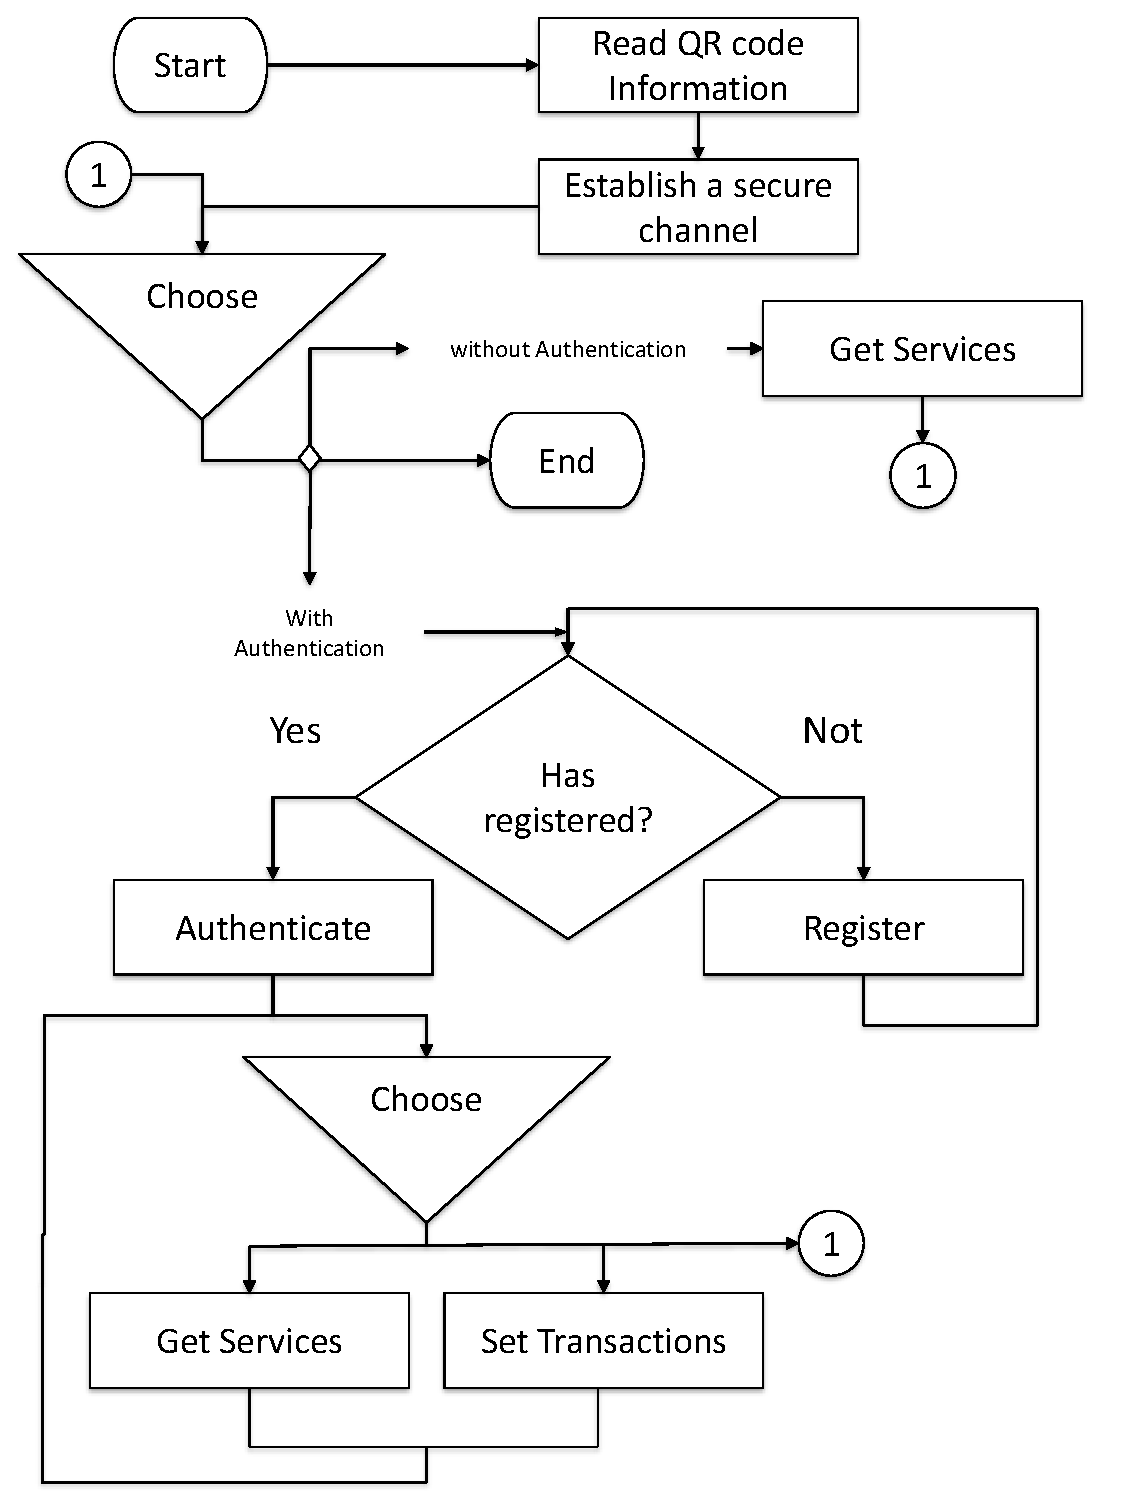
\includegraphics[scale=0.4]{images/dfd.pdf}
        \caption{General DFD about consuming services and set transactions}
    \label{fig:dfdForAuthServices}
 % \end{center}
\end{figure}

\subsection{Getting services without authentication}
\label{ssec:getServNoAuth}

Table~\ref{table:ProtGetServicesNoAuth} describes the process in
Alice and Bob notation, the explanation is as follows:  
\begin{itemize}
  \item  The initial knowledge consists in all values learned by the client and the miner 
        after completed the secure channel stage.
   \item The request of a service consists in sending an identity $C$, the data of the $QR$ code, and a 
        number $n$ denoting the number of service that is requested to be consumed. 
        The client ciphers  these messages using the secret key $K_{C\Server}$ obtained in
        the secure channel stage (see Section~\ref{sec:secureChannel}).
   \item The miner verifies if such a service can be consumed (according permissions) and then, 
        returns the answer $d$; ciphered using, again, the secret key $K_{C\Server}$.
\end{itemize}


\begin{table}[htb]
\footnotesize
\begin{center}
\caption{Get Service Protocol, authentication is not required}
\label{table:ProtGetServicesNoAuth}
\begin{tabular}{|l|}
\hline
           Initial Knowledge                                                             \\
            $C:C\lnk QR \lnk  K_{C\Server}$                                    \\
            $\Server: \Server\lnk K_{C\Server}$    \\ \hline \hline 
           Get a service                                                                        \\
           1.-$\Client\rightarrow \Server: \fat{C \lnk QR \lnk n}_{K_{C\Server}}$          \\ 
           \hspace{5mm} $d=getService(QR,n)$                                  \\  
           2.-$\Server\rightarrow \Client: \fat{C \lnk d}_{K_{C\Server}}$       \\  \hline \hline
\end{tabular}
\end{center}
\end{table}
\normalsize


\subsection{Get Services with authentication}
\label{ssec:ServAuth}
Sometimes it will be necessary to know who is consuming some services; for that, client and
miner are required to be authenticated. The authentication procedure requires a \textit{username} 
and a \textit{password}, which are developed after the \textit{registration process}. 


\subsubsection{Client Registration Process}
\label{sec:Registration}

This part consists in to establish a \textit{username} and a \textit{password}, which
will be mapped with an identity. The \textit{username} must be a valid email and the 
\textit{password} will be created by the user.

Table~\ref{table:reqSessKey} summarizes the protocol
in Alice\&Bob notation, its description is as follows: 
\begin{itemize}
  \item Firstly, the user must establish a secure channel with the miner 
    (see Section~\ref{sec:secureChannel}). In this step all exchanged messages are ciphered 
    using the symmetric key $K_{C\Server}$, which was obtained during the TLS protocol. 
  \item Secondly, the user must generate
    his username and password through the following steps:
    \begin{itemize}
    \item \textbf{First step:} the client sends his username denoted with his email $@$, and  
        a list of personal data $Pd$. 
    \item \textbf{Second step:} the server sends back the user via an email server $\Client_e$ a 
        data obtained of the client's personal information, $Pd$ and a challenge $X=f(Pd)$. 
    \item \textbf{Third step:} then, the client must generate the final password $P$, but
      only the hash is sent, $Hash(P,X)$.  Sending $Hash(P,X)$, we can
      ensure that $P$ will be only known by $\Client$.  
    \end{itemize}
  \item Finally, the miner creates a public and private key for the client ($K_{pub(\Client)}$ 
        and $K_{priv(\Client)}$), which the system maps with the client and the hashed password. 
        Note that, such public and private keys are unknown directly by $\Client$. 
\end{itemize}

\begin{table}[htb]
\footnotesize
\begin{center}
\caption{Client registration process}
\label{table:reqSessKey}
\begin{tabular}{|l|}
\hline
%{\bf Process}                                                                \\\hline\hline
%Initial Knowledge                                                             \\
%$C:N_{C}\lnk K_{pub(S)}\lnk N'_{C} \lnk K'_{CS}$                              \\
%$\ServerW: K_{pub(S)}\lnk K_{priv(S)}\lnk \ServerW\lnk N_{C}\lnk N_{C'}\lnk 
%                      K'_{CS}$                                                \\ \hline \hline
Initial Knowledge                                                             \\
$\Client:K_{C\ServerW}\lnk [@::Pd]$                                                    \\
$\ServerW: K_{C\ServerW}$                                                            \\ \hline \hline
1.-$\Client\rightarrow \ServerW:\fat{[@::Pd]}_{K_{\Client\ServerW}}$                     \\
\hspace{5mm} $X=f(Pd) $                           \\ 
2.-$\ServerW\rightarrow \Client_e: \fat{@\lnk Pd \lnk X}_{K_{\Client_e\ServerW}} $                  \\ 
\hspace{5mm} $\Client$ generates password $P$                          \\  
3.-$\Client\rightarrow \ServerW:\fat{@\lnk Hash(P,X)}_{K_{\Client\ServerW}}$                 \\  
\hspace{5mm} $\ServerW$ generates a pair key ($K_{pub(\Client)}$ and $K_{priv(\Client)}$)\\
\hspace{5mm} $\ServerW$ generates a block $bp = blockPubKey(K_{pub(\Client)})$\\
4.-$\ServerW\rightarrow [\Server_i .. \Server_n]: \fat{\ServerW \lnk bp}_{K_{\Server_i .. \Server_n}}$  \\  
5.-$\ServerW\rightarrow \Client: \fat{C \lnk K_{pub(\Client)}\lnk K_{priv(\Client)}}_{K_{\Server}}$          \\            \hline
New Knowledge Accumulated                                                     \\
$\Client:P\lnk X \lnk K_{pub(\Client)}\lnk K_{priv(\Client)}$                                                                \\
$\ServerW: K_{pub(\Client)}\lnk K_{priv(\Client)}\lnk X \lnk Hash(P,X)\lnk [@::Pd]$       \\\hline \hline 
\end{tabular}
\end{center}
\end{table}
\normalsize




The security properties the protocol must provides are: $P$ to be
known only by $C$; $K_{pub(\Client)}$ and $K_{priv(\Client)}$ to be known by $\Server$; 
and obtain strong authentication between the participants.

% We have verified this protocol using The AVISPA Tool Web
% Interface, available via http://www.avispa-project.org/
% finding the following:
% \begin{itemize}
%     \item The protocol provides secrecy.
%     \item We have proved that the protocol provides
%       \emph{authentication} from the client to the server on message 
%       $f(Pd)$ and \emph{weak authentication} from the server to the
%       client on message $Hash(P)$.
%     \item When we proved \emph{strong authentication}, it failed due
%       to the lack of freshness property generating The Dolev and Yao
%       attacker (of AVISPA tool) a replay attack. However, this attack
%       is already not possible when we consider that $K'_{CS}$ is
%       fresh, which was obtained in an immediately previous step. Even
%       though, we could include timestamps in all steps, however, that
%       is not necessary. 
% \end{itemize}

\subsubsection{Client-Miner Authentication}
\label{ssec:SecAuth}


The authentication process trusts in the users' \textit{username} 
(email) and \textit{password}, so, it is responsibility for the user 
to ensure his secrets. However, it is well known that any system 
cannot trust only in a user and password control access, because of that, 
it is important not only to encrypt the sensible information, but also
to implement more security mechanisms (like authentication procedure) to 
avoid possible attacks.

The goal of this stage is to establish authentication between a client and 
a miner after having a secure tunneling. Table~\ref{table:AuthProtocol} 
describes the authentication part and the explanation is as follows:

\begin{itemize}
  \item Both the client and the miner store all knowledge accumulated
    of previous steps. It is considered to have established a secure tunneling 
    with the miner using the TLS protocol and to have obtained the register
    procedure. So, the initial knowledge of the client consists in to know 
    the session key $K_{\Client\Server}$, his password $P$ and the secret $X$. 
    On the other hand, the miner knows the same session key, the client public and
    private key, personal information of the client, secret $X$ and the hashed 
    $Hash(P,X)$. The following steps are proposed:
    \begin{itemize}
    \item \textbf{First step:} the client sends a challenge to the
      miner $N_\Client$. The miner can map $@$ with $\Client$ and build $hash(@\lnk\Client\Server\lnk N_\Client)$. This message is ciphered with $K_{\Client\Server}$ because the session key has been destined for them. 
    \item \textbf{Second step:} the server responds to the client with a new challenge,
      firstly includes the client name $C$ (which is mapped with $@$) and a hashed message
      composed by $N_{\Client}$ and $X$ both messages must be known by the client. Again,
      all ciphered with $K_{\Client\Server}$.
    \item \textbf{Third step:} Once the client has accepted the previous step, it means that
      he has deduced all previous messages and he has authenticated to the miner, so, the 
      client sends back his username $@$, the challenge response $N_\Client$ as a freshness
      property and his password concatenated with $P$, $X$ and $N_{\Client}$.
  \end{itemize}
\item Finally, after having run the protocol it is expected to obtain strong authentication
    between the client and the miner. 
\end{itemize}
 
\begin{table}[htb]
\footnotesize
\begin{center}
\caption{Authentication Protocol}
\label{table:AuthProtocol}
\begin{tabular}{|l|l|l|}
\hline
{\bf Process}                                                                     \\\hline\hline
            Initial Knowledge                                                     \\
            $\Client:P\lnk X \lnk K_{\Client\Server}$                               \\
            \hspace{5mm}                                                 \\ 
            $\Server: K_{pub(\Client)}\lnk K_{priv(\Client)}\lnk Hash(P,X)\lnk X \lnk[@::Pd] \lnk K_{\Client\Server}$ \\\hline \hline
            Authentication                                                         \\
            1.-$\Client\rightarrow \Server: \fat{\Server \lnk @ \lnk N_{\Client} \lnk 
                                              Hash(@\lnk \Client \lnk \Server \lnk N_\Client)}_{K_{\Client\Server}}$  \\ 
            2.-$\Server\rightarrow \Client: \fat{\Client \lnk hash(N_{\Client},X)}_{K_{\Client\Server}}$ \\ 
            \hspace{5mm} $Y=hash(N_{\Client},hash(P,X))$                          \\              
            3.-$\Client\rightarrow \Server: \fat{@\lnk N_{\Client}\lnk Y}_{K_{\Client\Server}}$            \\ \hline  \hline
            New Knowledge Accumulated                                               \\
            $\Client: \Server \lnk N_\Client \lnk Y$         \\
            \hspace{5mm}                \\ 
            $\Server: \Client  \lnk N_\Client \lnk Y$          \\ 
            \hspace{5mm}                             \\ \hline \hline
\end{tabular}
\end{center}
\end{table}
\normalsize



\subsubsection{Get Services with authentication}
\label{ssec:getServAuth}


\begin{table}[htb]
\footnotesize
\begin{center}
\caption{Get Service Protocol with authentication}
\label{table:ProtGetServicesAuth}
\begin{tabular}{|l|}
\hline
           Initial Knowledge                                                             \\
            $C:C\lnk QR \lnk  K_{C\Server} \lnk Y$                                    \\
            $\Server: \Server\lnk K_{C\Server} \lnk Y$    \\ \hline \hline 
           Get a service                                                                        \\
           1.-$\Client\rightarrow \Server: \fat{C \lnk QR \lnk n \lnk Y}_{K_{C\Server}}$          \\ 
           \hspace{5mm} $d=getService(QR,n)$                                  \\  
           2.-$\Server\rightarrow \Client: \fat{C \lnk d \lnk Y}_{K_{C\Server}}$       \\  \hline \hline
\end{tabular}
\end{center}
\end{table}
\normalsize





\subsection{Set Transactions} 
\label{ssec:setTrans}

As shown by Table~\ref{table:ProtSetTrans} the participants in a transaction 
are the client and a miner.
The client knows the $QR$ code through a scan process with
a car; a secret shared key $K_{\Client\Server}$ established with
a miner in the secure channel process; a proof to have been authenticated
with the miner $N_{\Client\Server}$; and the transaction $T$ that client wish 
to do  (see Table~\ref{table:operations} for types of operations). 
The miner obviously knows also $K_{\Client\Server}$ and $N_{\Client\Server}$. 
\begin{enumerate}
    \item The protocol starts when the client $\Client$ builds the transaction 
        data $t$, the signature of the transaction $\fat{t}_{K_{priv(C)}}$ and sends
        all to the miner $\Server$; all ciphered with the 
        session key $K_{\Client\Server}$.
        The transaction data $t$, using function $setTransaction(\QR,T,N_{\Client\Server})$, 
        is constituted as follows:
        
        \begin{tabular}{lll}
                &               & \\ 
            \{  &               &    \\
                & registered:   & "true" 
                & plate:        & "LVP6598", \\
                & id:           & "1FMYU02Z97KA580G2", \\
                & timestamp:    & "18/09/2018 9:16:34am", \\
                & nonce:         & $N_{\Client\Server}$, \\
                & pubKey:       & $K_{pub(X)}$, \\
                & miner:        & M, \\
                & client:       & C, \\
                & transaction:  & T=$\fat{operation}_{priv(X)}$ \\
            \}  &               &   \\
        \end{tabular}
        
        Both \textit{plate} and \textit{id} are used to identify the car, 
        \textit{timestamp} used to identify the time, $N_{\Client\Server}$
        used to distinguish the session; the public key $K_{pub(X)}$
        of the next owner client, it could be the own $\Client$ or another
        owner;
        \textit{miner} and 
        \textit{client} fields to identify the participants in the transaction; 
        and $T$ stating
        what kind of operation is carrying out (see Table~\ref{table:operations}).
    \item Having the miner accepted the previous message (verifying the  
        session with $N_{\Client\Server}$ and all received messages), he proceeds to build 
        the block $b$ and broadcasts it to all miners $\Server\rightarrow [\Server_i .. \Server_n]$
        in order to execute a mining process; 
        this message is ciphered under \hl{the Ethereum plataform...}
        Block $b$ is as follows:
        \begin{tabular}{lll}
                &               & \\ 
            \{  &               &    \\
                & dataTran:     & t,  \\
                & previousHash: & "000dc75a3...7cf", \\
                & hash:         & "000d20368...1b8",\\
                & blockId:      & 1,\\
                & nonce:        & "42543524",\\
                & timestamp:    & "18/09/2018 9:40:44am" \\
            \}  &               &   \\
        \end{tabular}
        
    \item The miner solving the challenge $\Server_x$, returns again the block, $b'$, 
        but now it is mined. 
    \item Within the \hl{Ethereum Network} there exists a parity node\footnote{
            A parity node is a miner that is close with another and they have usual
            peer to peer communication.
        } to the miner $\Server$
        who also accepts the new block $b'$.
    \item Finally, the miner responds $r$ to the client as a proof that the transaction 
        was carried out successfully.
\end{enumerate}

\begin{table}[htb]
\footnotesize
\begin{center}
\caption{Set Transactions Protocol, authentication required}
\label{table:ProtSetTrans}
\begin{tabular}{|l|}
\hline
           Initial Knowledge                                                             \\
            $C:C\lnk QR \lnk  K_{C\Server} \lnk N_{\Client\Server} \lnk T$               \\
            $\Server: \Server\lnk K_{C\Server} \lnk N_{\Client\Server}$    \\ \hline \hline 
           Set a transaction                                                                        \\
           \hspace{5mm} $t=setTransaction(QR,T,N_{\Client\Server})$                                  \\  
           1.-$\Client\rightarrow \Server: \fat{C \lnk t \lnk \fat{t}_{K_{priv(C)}}}_{K_{C\Server}}$          \\ 
           \hspace{5mm} $b=block(t)$                                  \\  
           2.-$\Server\rightarrow [\Server_i .. \Server_n]: \fat{C \lnk b \lnk N_\Server}_{K_{\Server_i .. \Server_n}}$          \\ 
           \hspace{5mm} $b'=mine(b)$                                  \\  
           3.-$\Server_x\rightarrow [\Server_i .. \Server_n]: \fat{C \lnk b'}_{K_{\Server_i .. \Server_n}}$          \\            
           \hspace{5mm} $r=f(t)$                                  \\  
           4.-$\Server\rightarrow \Client: \fat{C \lnk r \lnk N_{\Client\Server}}_{K_{C\Server}}$       \\  \hline \hline
\end{tabular}
\end{center}
\end{table}
\normalsize
 %added by JC  ---
        \section{Transactions}


\subsection{Roles}

According to the permissions the users will have five defined roles: 
\textbf{U}ser,
\textbf{D}ealership,
\textbf{O}wner,
\textbf{G}overnment, and
\textbf{H}elper.
Each user could hold one or more roles.
Table \ref{table:operations} pinpoints the type of operations that each role can do and the explanation
is as follows: 
\begin{itemize}
    \item Any \textbf{U}ser will have enough permissions to interact with the system in order to 
        obtain information on the vehicle (Section~\ref{sec:getServices}). This role is also able 
        to buy cars, but it must be authenticated. 
        These permissions will be granted to the user once he has established the secure channel. 
    \item The \textbf{D}ealership is able to manufacture vehicles because of that he is who creates the 
        genesis block.
    \item Every car will have one and only one \textbf{O}wner at a given time. The owner will be the only one 
        that has permission to trade ownership, but also to request to the government to change legal
        status. In addition, he can request and authorize to \textbf{H}elper to add some information 
        about a car.
    \item \textbf{G}overnment will have the ability to  \textit{change legal status} when the 
        vehicle is involved in legal situations. For that, it will be necessary to establish 
        different status: \textit{stolen}, \textit{arrested}, \textit{penalty}, \textit{registered owner}, \textit{plate}, 
        \textit{tax history}, etc.
    \item The \textbf{H}elper role is who receives a temporal permission from the \textbf{O}wner to set one 
        transaction on the block-chain. The time frame for the temporal permission will be authorized by 
        the \textbf{O}wner of the car. The car owner will set a special transaction to give the helper 
        the permission. The helper role will be used for transactions that change one or more data of the 
        car's properties. This will include official services, mechanical adjustments, big aesthetic 
        modifications and insurance payments.
\end{itemize}







\begin{table}[htb]
\footnotesize
    \begin{center}
    \caption{Type of operation grouped by corresponding transactions}
    \label{table:operations}
        \begin{tabular}{|l|l|l|l|l|l|}
        \hline
        \textbf{Operation}          &\textbf{U}& \textbf{D}&\textbf{O}& \textbf{G}& \textbf{H}\\ \hline\hline
        Create (genesis block)      &          & X         &          &           &           \\ \hline\hline
        get information             & X        &           &          &           &           \\ \hline\hline
        sell                        &          &           & X        &           &           \\ \hline
        buy                         & X        &           &          &           &           \\ \hline\hline
        request change legal status &          &           & X        &           &           \\ \hline
        change legal status         &          &           &          & X         &           \\ \hline\hline
        request to add information  &          &           & X        &           &           \\ \hline
        add information             &          &           &          &           & X         \\ \hline
        authorize add information   &          &           & X        &           &           \\ \hline
        \end{tabular}
    \end{center}
\end{table} %added by JC


\subsection{Set Transactions} 
\label{ssec:setTrans}

As shown by Table~\ref{table:ProtSetTrans} the participants in a transaction 
are the client and a miner.
The client knows the $QR$ code through a scan process with
a car; a secret shared key $K_{\Client\Server}$ established with
a miner in the secure channel process; a proof to have been authenticated
with the miner $N_{\Client\Server}$; and the transaction $T$ that client wish 
to do  (see Table~\ref{table:operations} for types of operations). 
The miner obviously knows also $K_{\Client\Server}$ and $N_{\Client\Server}$. 
\begin{enumerate}
    \item The protocol starts when the client $\Client$ builds the transaction 
        data $t$, the signature of the transaction $\fat{t}_{K_{priv(C)}}$ and sends
        all to the miner $\Server$; all ciphered with the 
        session key $K_{\Client\Server}$.
        The transaction data $t$, using function $setTransaction(\QR,T,N_{\Client\Server})$, 
        is constituted as follows:
        
        \begin{tabular}{lll}
                &               & \\ 
            \{  &               &    \\
                & registered:   & "true" 
                & plate:        & "LVP6598", \\
                & id:           & "1FMYU02Z97KA580G2", \\
                & timestamp:    & "18/09/2018 9:16:34am", \\
                & nonce:         & $N_{\Client\Server}$, \\
                & pubKey:       & $K_{pub(X)}$, \\
                & miner:        & M, \\
                & client:       & C, \\
                & transaction:  & T=$\fat{operation}_{priv(X)}$ \\
            \}  &               &   \\
        \end{tabular}
        
        Both \textit{plate} and \textit{id} are used to identify the car, 
        \textit{timestamp} used to identify the time, $N_{\Client\Server}$
        used to distinguish the session; the public key $K_{pub(X)}$
        of the next owner client, it could be the own $\Client$ or another
        owner;
        \textit{miner} and 
        \textit{client} fields to identify the participants in the transaction; 
        and $T$ stating
        what kind of operation is carrying out (see Table~\ref{table:operations}).
    \item Having the miner accepted the previous message (verifying the  
        session with $N_{\Client\Server}$ and all received messages), he proceeds to build 
        the block $b$ and broadcasts it to all miners $\Server\rightarrow [\Server_i .. \Server_n]$
        in order to execute a mining process; 
        this message is ciphered under \hl{the Ethereum plataform...}
        Block $b$ is as follows:
        \begin{tabular}{lll}
                &               & \\ 
            \{  &               &    \\
                & dataTran:     & t,  \\
                & previousHash: & "000dc75a3...7cf", \\
                & hash:         & "000d20368...1b8",\\
                & blockId:      & 1,\\
                & nonce:        & "42543524",\\
                & timestamp:    & "18/09/2018 9:40:44am" \\
            \}  &               &   \\
        \end{tabular}
        
    \item The miner solving the challenge $\Server_x$, returns again the block, $b'$, 
        but now it is mined. 
    \item Within the \hl{Ethereum Network} there exists a parity node\footnote{
            A parity node is a miner that is close with another and they have usual
            peer to peer communication.
        } to the miner $\Server$
        who also accepts the new block $b'$.
    \item Finally, the miner responds $r$ to the client as a proof that the transaction 
        was carried out successfully.
\end{enumerate}

\begin{table}[htb]
\footnotesize
\begin{center}
\caption{Set Transactions Protocol, authentication required}
\label{table:ProtSetTrans}
\begin{tabular}{|l|}
\hline
           Initial Knowledge                                                             \\
            $C:C\lnk QR \lnk  K_{C\Server} \lnk N_{\Client\Server} \lnk T$               \\
            $\Server: \Server\lnk K_{C\Server} \lnk N_{\Client\Server}$    \\ \hline \hline 
           Set a transaction                                                                        \\
           \hspace{5mm} $t=setTransaction(QR,T,N_{\Client\Server})$                                  \\  
           1.-$\Client\rightarrow \Server: \fat{C \lnk t \lnk \fat{t}_{K_{priv(C)}}}_{K_{C\Server}}$          \\ 
           \hspace{5mm} $b=block(t)$                                  \\  
           2.-$\Server\rightarrow [\Server_i .. \Server_n]: \fat{C \lnk b \lnk N_\Server}_{K_{\Server_i .. \Server_n}}$          \\ 
           \hspace{5mm} $b'=mine(b)$                                  \\  
           3.-$\Server_x\rightarrow [\Server_i .. \Server_n]: \fat{C \lnk b'}_{K_{\Server_i .. \Server_n}}$          \\            
           \hspace{5mm} $r=f(t)$                                  \\  
           4.-$\Server\rightarrow \Client: \fat{C \lnk r \lnk N_{\Client\Server}}_{K_{C\Server}}$       \\  \hline \hline
\end{tabular}
\end{center}
\end{table}
\normalsize
 %added by JC  ---
        %\input{sections/secGetServAuth} %added by JC  ---
        \input{sections/secSetTransactions} %added by JC  ---

       % \section{Related Work}

        
        
\section{Conclusion}
The conclusion goes here.

        % if have a single appendix:
%\appendix[Proof of the Zonklar Equations]
% or
%\appendix  % for no appendix heading
% do not use \section anymore after \appendix, only \section*
% is possibly needed

% use appendices with more than one appendix
% then use \section to start each appendix
% you must declare a \section before using any
% \subsection or using \label (\appendices by itself
% starts a section numbered zero.)
%


%\appendices
%\section{Proof of the First Zonklar Equation}
%Appendix one text goes here.

% you can choose not to have a title for an appendix
% if you want by leaving the argument blank
%\section{}
%Appendix two text goes here.

        
% use section* for acknowledgment
\ifCLASSOPTIONcompsoc
  % The Computer Society usually uses the plural form
  \section*{Acknowledgments}
\else
  % regular IEEE prefers the singular form
  \section*{Acknowledgment}
\fi


The authors would like to thank...



        % Can use something like this to put references on a page
% by themselves when using endfloat and the captionsoff option.
\ifCLASSOPTIONcaptionsoff
  \newpage
\fi



% trigger a \newpage just before the given reference
% number - used to balance the columns on the last page
% adjust value as needed - may need to be readjusted if
% the document is modified later
%\IEEEtriggeratref{8}
% The "triggered" command can be changed if desired:
%\IEEEtriggercmd{\enlargethispage{-5in}}

% references section

% can use a bibliography generated by BibTeX as a .bbl file
% BibTeX documentation can be easily obtained at:
% http://mirror.ctan.org/biblio/bibtex/contrib/doc/
% The IEEEtran BibTeX style support page is at:
% http://www.michaelshell.org/tex/ieeetran/bibtex/
\bibliographystyle{IEEEtran}
% argument is your BibTeX string definitions and bibliography database(s)
\bibliography{bib/paper}

\nocite{*}

% biography section
% 
% If you have an EPS/PDF photo (graphicx package needed) extra braces are
% needed around the contents of the optional argument to biography to prevent
% the LaTeX parser from getting confused when it sees the complicated
% \includegraphics command within an optional argument. (You could create
% your own custom macro containing the \includegraphics command to make things
% simpler here.)
%\begin{IEEEbiography}[{\includegraphics[width=1in,height=1.25in,clip,keepaspectratio]{mshell}}]{Michael Shell}
% or if you just want to reserve a space for a photo:

%\begin{IEEEbiography}{Juan-Carlos L\'opez-Pimentel}
%Biography text here.
%\end{IEEEbiography}


\begin{IEEEbiographynophoto}{Juan-Carlos L\'opez-Pimentel}
was born in Tuxtla Guti\'errez, Mexico. He holds a PhD and Master in Computer Science, both from the Tecnológico de Monterrey Campus Estado de Mexico. He has a Bachelor in Computer Systems Engineering from Institute of Technology in Tuxtla Gutierrez (in 2001). He was distinguished for being part of the Mexican National System of Researchers (2010-2013), Level C. His research interest is about Computer Security, Distributed Systems and Software Development. Currently he is a Research Professor at Universidad Panamericana, Campus Guadalajara.
\end{IEEEbiographynophoto}


% if you will not have a photo at all:
\begin{IEEEbiographynophoto}{Miguel Alcaraz}
Biography text here.
\end{IEEEbiographynophoto}
was born in Zapopan, Mexico. He received an MS degree in Optics in 2006 and his PhD in 2011 from Instituto Nacional de Astrofisica Optica y Electronica. At present, he works in the Engineering Department at Universidad Panamericana, Mexico. His research interests are focused on security and social networking.
% insert where needed to balance the two columns on the last page with
% biographies
%\newpage

\begin{IEEEbiographynophoto}{Leonardo J. Valdivia}
was born in Guadalajara, Mexico, in 1988. He received an MS degree in Telecommunications Engineering in 2014 and his PhD in 2017 from the University of Navarras School of Engineering (TECNUN).After spending 3 years working on software for the automotive sector and four years for railway sector, in 2017, he joined the Engineering Area at Universidad Panamericana. At present, his research interests are focused on safety and security interaction.
\end{IEEEbiographynophoto}


\begin{IEEEbiographynophoto}{Carolina del Valle Soto}
was born in Medellin, Colombia. She has a PhD. in Information Technology and Communications with a doctoral dissertation: Design, implementation and comparison of a new routing protocol for Wireless Sensor Networks. She studied a Master in Science of electronic engineering (Telecommunications) with a thesis named Development of a P2P network with DNS security. Carolina has a Bachelor in electronic engineering with a thesis in Design and construction of a photon counting systems. Carolina´s main skills in to apply and develop in the areas of telecommunications, specifically wired and wireless networks, programming and security. Carolina belongs to the National Research System, level C.
\end{IEEEbiographynophoto}


% You can push biographies down or up by placing
% a \vfill before or after them. The appropriate
% use of \vfill depends on what kind of text is
% on the last page and whether or not the columns
% are being equalized.

%\vfill

% Can be used to pull up biographies so that the bottom of the last one
% is flush with the other column.
%\enlargethispage{-5in}



% that's all folks

\end{document}


